\documentclass{beamer}
\usetheme[subsectionpage=progressbar,
		  progressbar=frametitle,
		  % background=dark
		 ]{metropolis}

\usepackage{media9}
		 
\title{Taller Básico de Impresión 3D}
\date{\today}
\author{Idir Expósito Gómez}
\institute{Málaga MakerSpace}
\begin{document}
	\maketitle
	
	%%%%%%%%%%%%%%%%%%%%%%%%%%%%%%%%%%%%%%%%
	\section{Introducción}
	
	\subsection{Qué es el Málaga MakerSpace}
	
	\subsection{Objetivos de este taller}
	\begin{frame}{Competencias generales}
		\begin{itemize}
			\item Entender los principios físicos de la impresión 3D.
			\item Reconocer qué se puede fabricar con esta tecnología.
			\item Conocer las partes físicas de una impresora y su función.
			\item Conocer los principios del rebanado (slicing).
		\end{itemize}
	\end{frame}
	\begin{frame}{Competencias específicas}
		\begin{itemize}
			\item Ajustar los parámetros más importantes con Ultimaker CURA.
			\item Conocer la impresora Creality CR-10 y su calibrado.
			\item Conocer los problemas de impresión más comunes y cómo solventarlos.
			\item Conocer las reglas de impresión en el Málaga MakerSpace.
		\end{itemize}
	\end{frame}
	
	\subsection{Sistema de impresión en el MMS}
	\begin{frame}{Reglas}
		\begin{enumerate}
			\item Obligatorio superar este taller.
			\item Solo impresión con PLA y mantenimiento básico.
			\item Siempre debe haber supervisión de la impresión.
			\item No desatender la impresora si no se puede controlar remotamente.
			\item Respetar legislación de derechos de autor.
			\item Uso responsable de la maquinaria y responsabilización de los errores.
			\item Prohibido modificar la maquinaria.
			\item Obligatoria reserva de maquinaria y material.
			\item El pago se realiza por adelantado.
			\item Se pueden realizar trabajos para terceros con autorización previa.
		\end{enumerate}
	\end{frame}
	\begin{frame}[standout]{Costes}
		El sistema de costes es provisional mientras no haya cuota de membresía y espacio físico.
	\end{frame}
	\begin{frame}{Costes para personas no cualificadas}
		\begin{enumerate}
			\item 0.03€ por gramo de PLA.
			\item 0.25€ por hora de impresión, en intervalos de media hora.
			\item 5€ por hora de trabajo humano.
			\item 10\% adicional por fallos.
			\item 21\% de IVA.
		\end{enumerate}
		$$\text{Coste}=1.21\times 1.1\times \left( 5\times \text{Operario} +0.25\times\text{Horas}+0.03\times\text{Gramos} \right)$$
	\end{frame}
	\begin{frame}{Costes para personas cualificadas sin material}
		\begin{enumerate}
			\item 0.03€ por gramo de PLA.
			\item 0.25€ por hora de impresión, en intervalos de media hora.
			\item 21\% de IVA.
		\end{enumerate}
		$$\text{Coste}=1.21\times \left( 0.25\times\text{Horas}+0.03\times\text{Gramos} \right)$$
	\end{frame}
	\begin{frame}{Costes para personas cualificadas con material}
		\begin{enumerate}
			\item 0.25€ por hora de impresión, en intervalos de media hora.
			\item 21\% de IVA.
		\end{enumerate}
		$$\text{Coste}=1.21\times \left( 0.25\times\text{Horas} \right)$$
	\end{frame}
	
	%%%%%%%%%%%%%%%%%%%%%%%%%%%%%%%%%%%%%%%%
	\section{Fundamentos de Modelado por Deposición Fundida (FDM)}
	\begin{frame}{Fundamentos de FDM}
		\begin{figure}
			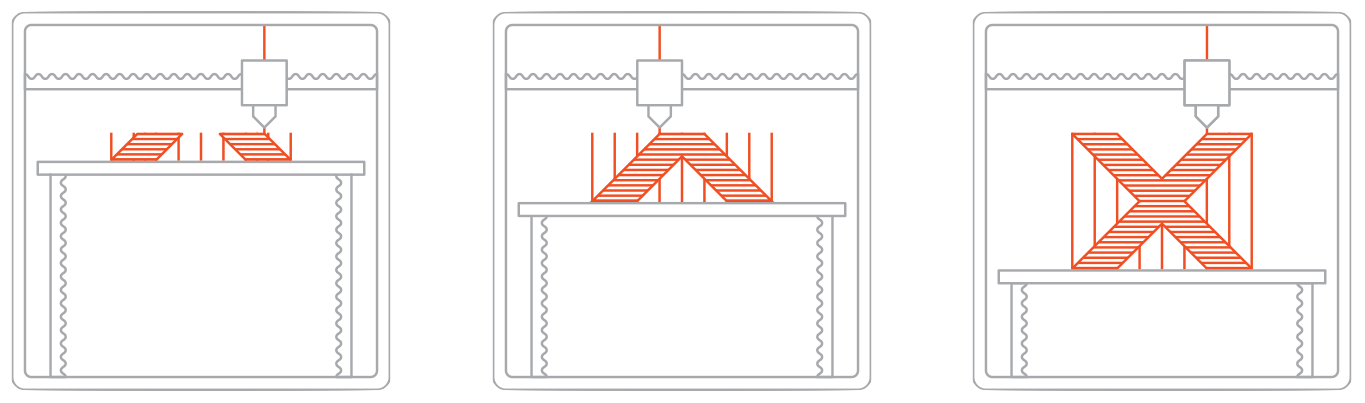
\includegraphics[width=\textwidth]{images/fdm}
			\caption{Proceso FDM}
		\end{figure}
	\end{frame}
	
	\subsection{Partes y características de una impresora}
	\begin{frame}{Placa madre}
		%TODO IMAGE
	\end{frame}
	\begin{frame}{Extrusor}
		%TODO IMAGE
	\end{frame}
	\begin{frame}{Cama de impresión}
		%TODO IMAGE
	\end{frame}
	\begin{frame}{Finales de carrera}
		%TODO IMAGE
	\end{frame}
	
	\subsection{Materiales}
	\begin{frame}{Ácido Poliláctico (PLA)}
		
	\end{frame}
	
	%%%%%%%%%%%%%%%%%%%%%%%%%%%%%%%%%%%%%%%%
	\section{Antes de imprimir}
	
	%%%%%%%%%%%%%%%%%%%%%%%%%%%%%%%%%%%%%%%%
	\section{Durante la impresión}
	
	%%%%%%%%%%%%%%%%%%%%%%%%%%%%%%%%%%%%%%%%
	\section{Tras la impresión}
\end{document}
